\documentclass[twoside]{book}

% Packages required by doxygen
\usepackage{fixltx2e}
\usepackage{calc}
\usepackage{doxygen}
\usepackage[export]{adjustbox} % also loads graphicx
\usepackage{graphicx}
\usepackage[utf8]{inputenc}
\usepackage{makeidx}
\usepackage{multicol}
\usepackage{multirow}
\PassOptionsToPackage{warn}{textcomp}
\usepackage{textcomp}
\usepackage[nointegrals]{wasysym}
\usepackage[table]{xcolor}

% Font selection
\usepackage[T1]{fontenc}
\usepackage[scaled=.90]{helvet}
\usepackage{courier}
\usepackage{amssymb}
\usepackage{sectsty}
\renewcommand{\familydefault}{\sfdefault}
\allsectionsfont{%
  \fontseries{bc}\selectfont%
  \color{darkgray}%
}
\renewcommand{\DoxyLabelFont}{%
  \fontseries{bc}\selectfont%
  \color{darkgray}%
}
\newcommand{\+}{\discretionary{\mbox{\scriptsize$\hookleftarrow$}}{}{}}

% Page & text layout
\usepackage{geometry}
\geometry{%
  a4paper,%
  top=2.5cm,%
  bottom=2.5cm,%
  left=2.5cm,%
  right=2.5cm%
}
\tolerance=750
\hfuzz=15pt
\hbadness=750
\setlength{\emergencystretch}{15pt}
\setlength{\parindent}{0cm}
\setlength{\parskip}{3ex plus 2ex minus 2ex}
\makeatletter
\renewcommand{\paragraph}{%
  \@startsection{paragraph}{4}{0ex}{-1.0ex}{1.0ex}{%
    \normalfont\normalsize\bfseries\SS@parafont%
  }%
}
\renewcommand{\subparagraph}{%
  \@startsection{subparagraph}{5}{0ex}{-1.0ex}{1.0ex}{%
    \normalfont\normalsize\bfseries\SS@subparafont%
  }%
}
\makeatother

% Headers & footers
\usepackage{fancyhdr}
\pagestyle{fancyplain}
\fancyhead[LE]{\fancyplain{}{\bfseries\thepage}}
\fancyhead[CE]{\fancyplain{}{}}
\fancyhead[RE]{\fancyplain{}{\bfseries\leftmark}}
\fancyhead[LO]{\fancyplain{}{\bfseries\rightmark}}
\fancyhead[CO]{\fancyplain{}{}}
\fancyhead[RO]{\fancyplain{}{\bfseries\thepage}}
\fancyfoot[LE]{\fancyplain{}{}}
\fancyfoot[CE]{\fancyplain{}{}}
\fancyfoot[RE]{\fancyplain{}{\bfseries\scriptsize Generated by Doxygen }}
\fancyfoot[LO]{\fancyplain{}{\bfseries\scriptsize Generated by Doxygen }}
\fancyfoot[CO]{\fancyplain{}{}}
\fancyfoot[RO]{\fancyplain{}{}}
\renewcommand{\footrulewidth}{0.4pt}
\renewcommand{\chaptermark}[1]{%
  \markboth{#1}{}%
}
\renewcommand{\sectionmark}[1]{%
  \markright{\thesection\ #1}%
}

% Indices & bibliography
\usepackage{natbib}
\usepackage[titles]{tocloft}
\setcounter{tocdepth}{3}
\setcounter{secnumdepth}{5}
\makeindex

% Hyperlinks (required, but should be loaded last)
\usepackage{ifpdf}
\ifpdf
  \usepackage[pdftex,pagebackref=true]{hyperref}
\else
  \usepackage[ps2pdf,pagebackref=true]{hyperref}
\fi
\hypersetup{%
  colorlinks=true,%
  linkcolor=blue,%
  citecolor=blue,%
  unicode%
}

% Custom commands
\newcommand{\clearemptydoublepage}{%
  \newpage{\pagestyle{empty}\cleardoublepage}%
}

\usepackage{caption}
\captionsetup{labelsep=space,justification=centering,font={bf},singlelinecheck=off,skip=4pt,position=top}

%===== C O N T E N T S =====

\begin{document}

% Titlepage & ToC
\hypersetup{pageanchor=false,
             bookmarksnumbered=true,
             pdfencoding=unicode
            }
\pagenumbering{alph}
\begin{titlepage}
\vspace*{7cm}
\begin{center}%
{\Large My Project }\\
\vspace*{1cm}
{\large Generated by Doxygen 1.8.12}\\
\end{center}
\end{titlepage}
\clearemptydoublepage
\pagenumbering{roman}
\tableofcontents
\clearemptydoublepage
\pagenumbering{arabic}
\hypersetup{pageanchor=true}

%--- Begin generated contents ---
\chapter{Template}
\label{md__r_e_a_d_m_e}
\hypertarget{md__r_e_a_d_m_e}{}
Visual Studio 2015 Templates 
\chapter{Hierarchical Index}
\section{Class Hierarchy}
This inheritance list is sorted roughly, but not completely, alphabetically\+:\begin{DoxyCompactList}
\item \contentsline{section}{C\+Base4618}{\pageref{class_c_base4618}}{}
\begin{DoxyCompactList}
\item \contentsline{section}{C\+Pong}{\pageref{class_c_pong}}{}
\end{DoxyCompactList}
\item \contentsline{section}{C\+Control}{\pageref{class_c_control}}{}
\item \contentsline{section}{Client}{\pageref{class_client}}{}
\item \contentsline{section}{Serial}{\pageref{class_serial}}{}
\item \contentsline{section}{Server}{\pageref{class_server}}{}
\end{DoxyCompactList}

\chapter{Class Index}
\section{Class List}
Here are the classes, structs, unions and interfaces with brief descriptions\+:\begin{DoxyCompactList}
\item\contentsline{section}{\hyperlink{class_c_base4618}{C\+Base4618} \\*C++ object used to hold common code used in all of the following labs for this course }{\pageref{class_c_base4618}}{}
\item\contentsline{section}{\hyperlink{class_c_control}{C\+Control} \\*C++ object used for communication with the embedded system }{\pageref{class_c_control}}{}
\item\contentsline{section}{\hyperlink{class_client}{Client} }{\pageref{class_client}}{}
\item\contentsline{section}{\hyperlink{class_c_pong}{C\+Pong} \\*C++ object used to create a Pong; }{\pageref{class_c_pong}}{}
\item\contentsline{section}{\hyperlink{class_serial}{Serial} }{\pageref{class_serial}}{}
\item\contentsline{section}{\hyperlink{class_server}{Server} }{\pageref{class_server}}{}
\end{DoxyCompactList}

\chapter{Class Documentation}
\hypertarget{class_c_base4618}{}\section{C\+Base4618 Class Reference}
\label{class_c_base4618}\index{C\+Base4618@{C\+Base4618}}


C++ object used to hold common code used in all of the following labs for this course.  




{\ttfamily \#include $<$C\+Base4618.\+h$>$}

Inheritance diagram for C\+Base4618\+:\begin{figure}[H]
\begin{center}
\leavevmode
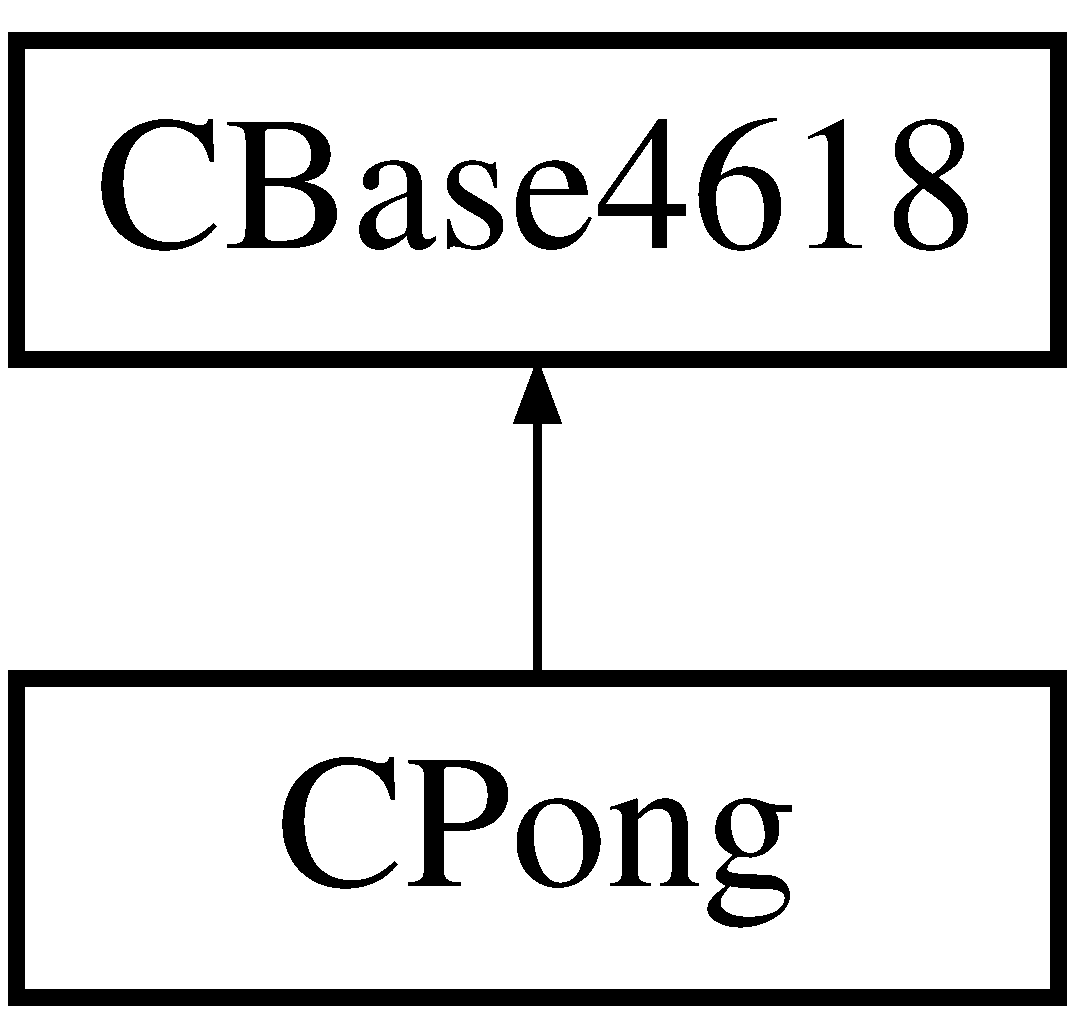
\includegraphics[height=2.000000cm]{class_c_base4618}
\end{center}
\end{figure}
\subsection*{Public Member Functions}
\begin{DoxyCompactItemize}
\item 
virtual void \hyperlink{class_c_base4618_ae1ac81eaa56ded6600262c361f723cb8}{update} ()
\begin{DoxyCompactList}\small\item\em Overloaded in C\+Sketch updates the coordinates. \end{DoxyCompactList}\item 
virtual void \hyperlink{class_c_base4618_a853327d563d064bb31db241861c4d291}{draw} ()
\begin{DoxyCompactList}\small\item\em Overloaded in C\+Sketch to draw. \end{DoxyCompactList}\item 
virtual void \hyperlink{class_c_base4618_a535e816d735d10d6048dd39cd893d393}{run} ()
\begin{DoxyCompactList}\small\item\em runs update and draw in an infinite loop until a button is pressed. \end{DoxyCompactList}\end{DoxyCompactItemize}
\subsection*{Public Attributes}
\begin{DoxyCompactItemize}
\item 
\hypertarget{class_c_base4618_aa07dc8a46156de408c94acf90f46043a}{}\label{class_c_base4618_aa07dc8a46156de408c94acf90f46043a} 
\hyperlink{class_c_control}{C\+Control} {\bfseries control}
\item 
\hypertarget{class_c_base4618_a1b925f757247b33ca2072f777f24582d}{}\label{class_c_base4618_a1b925f757247b33ca2072f777f24582d} 
cv\+::\+Mat {\bfseries \+\_\+canvas}
\end{DoxyCompactItemize}


\subsection{Detailed Description}
C++ object used to hold common code used in all of the following labs for this course. 

This class has a \hyperlink{class_c_control}{C\+Control} object and an Open cv object which are used in C\+Sketch class.\+There will also be three public methods which implement the two of which are overloaded in C\+Sketch.

\begin{DoxyAuthor}{Author}
Balkaran Sidhu 
\end{DoxyAuthor}


\subsection{Member Function Documentation}
\hypertarget{class_c_base4618_a853327d563d064bb31db241861c4d291}{}\label{class_c_base4618_a853327d563d064bb31db241861c4d291} 
\index{C\+Base4618@{C\+Base4618}!draw@{draw}}
\index{draw@{draw}!C\+Base4618@{C\+Base4618}}
\subsubsection{\texorpdfstring{draw()}{draw()}}
{\footnotesize\ttfamily void C\+Base4618\+::draw (\begin{DoxyParamCaption}{ }\end{DoxyParamCaption})\hspace{0.3cm}{\ttfamily [virtual]}}



Overloaded in C\+Sketch to draw. 


\begin{DoxyParams}{Parameters}
{\em N\+O\+N\+E.} & \\
\hline
\end{DoxyParams}
\begin{DoxyReturn}{Returns}
nothing to return 
\end{DoxyReturn}


Reimplemented in \hyperlink{class_c_pong_af43dbb61f1f1addd6920b01aeca3fa63}{C\+Pong}.

\hypertarget{class_c_base4618_a535e816d735d10d6048dd39cd893d393}{}\label{class_c_base4618_a535e816d735d10d6048dd39cd893d393} 
\index{C\+Base4618@{C\+Base4618}!run@{run}}
\index{run@{run}!C\+Base4618@{C\+Base4618}}
\subsubsection{\texorpdfstring{run()}{run()}}
{\footnotesize\ttfamily void C\+Base4618\+::run (\begin{DoxyParamCaption}{ }\end{DoxyParamCaption})\hspace{0.3cm}{\ttfamily [virtual]}}



runs update and draw in an infinite loop until a button is pressed. 


\begin{DoxyParams}{Parameters}
{\em N\+O\+N\+E.} & \\
\hline
\end{DoxyParams}
\begin{DoxyReturn}{Returns}
Nothing to return 
\end{DoxyReturn}
\hypertarget{class_c_base4618_ae1ac81eaa56ded6600262c361f723cb8}{}\label{class_c_base4618_ae1ac81eaa56ded6600262c361f723cb8} 
\index{C\+Base4618@{C\+Base4618}!update@{update}}
\index{update@{update}!C\+Base4618@{C\+Base4618}}
\subsubsection{\texorpdfstring{update()}{update()}}
{\footnotesize\ttfamily void C\+Base4618\+::update (\begin{DoxyParamCaption}{ }\end{DoxyParamCaption})\hspace{0.3cm}{\ttfamily [virtual]}}



Overloaded in C\+Sketch updates the coordinates. 


\begin{DoxyParams}{Parameters}
{\em None.} & \\
\hline
\end{DoxyParams}
\begin{DoxyReturn}{Returns}
nothing to return 
\end{DoxyReturn}


Reimplemented in \hyperlink{class_c_pong_a819c9942552ff12a11be284a89e3ab12}{C\+Pong}.



The documentation for this class was generated from the following files\+:\begin{DoxyCompactItemize}
\item 
C\+Base4618.\+h\item 
C\+Base4618.\+cpp\end{DoxyCompactItemize}

\hypertarget{class_c_control}{}\section{C\+Control Class Reference}
\label{class_c_control}\index{C\+Control@{C\+Control}}


C++ object used for communication with the embedded system.  




{\ttfamily \#include $<$C\+Control.\+h$>$}

\subsection*{Public Member Functions}
\begin{DoxyCompactItemize}
\item 
void \hyperlink{class_c_control_a96db7512a2239f017fc27354eb840abf}{init\+\_\+com} (int com)
\begin{DoxyCompactList}\small\item\em Sets the desired C\+OM port. \end{DoxyCompactList}\item 
bool \hyperlink{class_c_control_a08d481253181db60a8aec73583a1713f}{get\+\_\+data} (string mode, string type, string channel, int \&result)
\begin{DoxyCompactList}\small\item\em Gets data on a digital or analog channel. \end{DoxyCompactList}\item 
bool \hyperlink{class_c_control_a96b82a830c7dca2ee4fd66f5c04d0c9a}{set\+\_\+data} (string type, string channel, string val)
\begin{DoxyCompactList}\small\item\em S\+E\+Ts data on a digital channel. \end{DoxyCompactList}\item 
int \hyperlink{class_c_control_acf0620145af8af25d74656b0e66e8658}{get\+\_\+analog} (int value)
\begin{DoxyCompactList}\small\item\em Returns a percent scale value of the joystick position. \end{DoxyCompactList}\item 
int \hyperlink{class_c_control_afae6ad2b10c7afb9c627e7824f30ff42}{get\+\_\+button} ()
\begin{DoxyCompactList}\small\item\em Debounces the puch button. \end{DoxyCompactList}\item 
void \hyperlink{class_c_control_a1a643d9630738943580882ea97e4caec}{servo} ()
\begin{DoxyCompactList}\small\item\em Displayes servo position. \end{DoxyCompactList}\end{DoxyCompactItemize}
\subsection*{Public Attributes}
\begin{DoxyCompactItemize}
\item 
\hypertarget{class_c_control_ace18c1c2a9b70a663bad4ede2556a788}{}\label{class_c_control_ace18c1c2a9b70a663bad4ede2556a788} 
int \hyperlink{class_c_control_ace18c1c2a9b70a663bad4ede2556a788}{x}
\begin{DoxyCompactList}\small\item\em X value Jo\+Y\+S\+T\+I\+CK. \end{DoxyCompactList}\item 
\hypertarget{class_c_control_a143a30a147cb0e1487ff52a7ca1a937e}{}\label{class_c_control_a143a30a147cb0e1487ff52a7ca1a937e} 
int \hyperlink{class_c_control_a143a30a147cb0e1487ff52a7ca1a937e}{y}
\begin{DoxyCompactList}\small\item\em Y vakue J\+O\+Y\+S\+T\+I\+CK. \end{DoxyCompactList}\end{DoxyCompactItemize}


\subsection{Detailed Description}
C++ object used for communication with the embedded system. 

This class has a serial port object and an init\+\_\+com method which initializes the serial port to the com port passed as a parameter to the method.\+There will also be two public methods which implement the serial communication protocol

\begin{DoxyAuthor}{Author}
Balkaran Sidhu 
\end{DoxyAuthor}


\subsection{Member Function Documentation}
\hypertarget{class_c_control_acf0620145af8af25d74656b0e66e8658}{}\label{class_c_control_acf0620145af8af25d74656b0e66e8658} 
\index{C\+Control@{C\+Control}!get\+\_\+analog@{get\+\_\+analog}}
\index{get\+\_\+analog@{get\+\_\+analog}!C\+Control@{C\+Control}}
\subsubsection{\texorpdfstring{get\+\_\+analog()}{get\_analog()}}
{\footnotesize\ttfamily int C\+Control\+::get\+\_\+analog (\begin{DoxyParamCaption}\item[{int}]{value }\end{DoxyParamCaption})}



Returns a percent scale value of the joystick position. 


\begin{DoxyParams}{Parameters}
{\em integer} & value\+:raw value of joystick.\\
\hline
\end{DoxyParams}
\begin{DoxyReturn}{Returns}
returns percent scale value. 
\end{DoxyReturn}
\hypertarget{class_c_control_afae6ad2b10c7afb9c627e7824f30ff42}{}\label{class_c_control_afae6ad2b10c7afb9c627e7824f30ff42} 
\index{C\+Control@{C\+Control}!get\+\_\+button@{get\+\_\+button}}
\index{get\+\_\+button@{get\+\_\+button}!C\+Control@{C\+Control}}
\subsubsection{\texorpdfstring{get\+\_\+button()}{get\_button()}}
{\footnotesize\ttfamily int C\+Control\+::get\+\_\+button (\begin{DoxyParamCaption}{ }\end{DoxyParamCaption})}



Debounces the puch button. 


\begin{DoxyParams}{Parameters}
{\em none.} & \\
\hline
\end{DoxyParams}
\begin{DoxyReturn}{Returns}
nothing to return. 
\end{DoxyReturn}
\hypertarget{class_c_control_a08d481253181db60a8aec73583a1713f}{}\label{class_c_control_a08d481253181db60a8aec73583a1713f} 
\index{C\+Control@{C\+Control}!get\+\_\+data@{get\+\_\+data}}
\index{get\+\_\+data@{get\+\_\+data}!C\+Control@{C\+Control}}
\subsubsection{\texorpdfstring{get\+\_\+data()}{get\_data()}}
{\footnotesize\ttfamily bool C\+Control\+::get\+\_\+data (\begin{DoxyParamCaption}\item[{string}]{mode,  }\item[{string}]{type,  }\item[{string}]{channel,  }\item[{int \&}]{result }\end{DoxyParamCaption})}



Gets data on a digital or analog channel. 


\begin{DoxyParams}{Parameters}
{\em strings} & of Mode used to select G\+ET or S\+ET. \\
\hline
{\em strings} & of type used to select Digital,Analog or Servo. \\
\hline
{\em strings} & of channel used select the the channel to read from. \\
\hline
{\em strings} & of result passed by referance. \\
\hline
\end{DoxyParams}
\begin{DoxyReturn}{Returns}
returns T\+R\+UE or F\+A\+L\+SE 
\end{DoxyReturn}
\hypertarget{class_c_control_a96db7512a2239f017fc27354eb840abf}{}\label{class_c_control_a96db7512a2239f017fc27354eb840abf} 
\index{C\+Control@{C\+Control}!init\+\_\+com@{init\+\_\+com}}
\index{init\+\_\+com@{init\+\_\+com}!C\+Control@{C\+Control}}
\subsubsection{\texorpdfstring{init\+\_\+com()}{init\_com()}}
{\footnotesize\ttfamily void C\+Control\+::init\+\_\+com (\begin{DoxyParamCaption}\item[{int}]{com }\end{DoxyParamCaption})}



Sets the desired C\+OM port. 


\begin{DoxyParams}{Parameters}
{\em C\+OM} & port string. \\
\hline
\end{DoxyParams}
\begin{DoxyReturn}{Returns}
nothing to return 
\end{DoxyReturn}
\hypertarget{class_c_control_a1a643d9630738943580882ea97e4caec}{}\label{class_c_control_a1a643d9630738943580882ea97e4caec} 
\index{C\+Control@{C\+Control}!servo@{servo}}
\index{servo@{servo}!C\+Control@{C\+Control}}
\subsubsection{\texorpdfstring{servo()}{servo()}}
{\footnotesize\ttfamily void C\+Control\+::servo (\begin{DoxyParamCaption}{ }\end{DoxyParamCaption})}



Displayes servo position. 


\begin{DoxyParams}{Parameters}
{\em none.} & \\
\hline
\end{DoxyParams}
\begin{DoxyReturn}{Returns}
nothing to return. 
\end{DoxyReturn}
\hypertarget{class_c_control_a96b82a830c7dca2ee4fd66f5c04d0c9a}{}\label{class_c_control_a96b82a830c7dca2ee4fd66f5c04d0c9a} 
\index{C\+Control@{C\+Control}!set\+\_\+data@{set\+\_\+data}}
\index{set\+\_\+data@{set\+\_\+data}!C\+Control@{C\+Control}}
\subsubsection{\texorpdfstring{set\+\_\+data()}{set\_data()}}
{\footnotesize\ttfamily bool C\+Control\+::set\+\_\+data (\begin{DoxyParamCaption}\item[{string}]{type,  }\item[{string}]{channel,  }\item[{string}]{val }\end{DoxyParamCaption})}



S\+E\+Ts data on a digital channel. 


\begin{DoxyParams}{Parameters}
{\em strings} & of type used to select Digital,Analog or Servo. \\
\hline
{\em strings} & of channel used select the the channel to write to. \\
\hline
{\em strings} & of valued on a channel used select the the channel to write to. \\
\hline
\end{DoxyParams}
\begin{DoxyReturn}{Returns}
returns T\+R\+UE or F\+A\+L\+SE 
\end{DoxyReturn}


The documentation for this class was generated from the following files\+:\begin{DoxyCompactItemize}
\item 
C\+Control.\+h\item 
C\+Control.\+cpp\end{DoxyCompactItemize}

\hypertarget{class_client}{}\section{Client Class Reference}
\label{class_client}\index{Client@{Client}}
\subsection*{Public Member Functions}
\begin{DoxyCompactItemize}
\item 
\hypertarget{class_client_ae48ea283b08db8a87601a96690895a21}{}\label{class_client_ae48ea283b08db8a87601a96690895a21} 
{\bfseries Client} (int port, std\+::string addr)
\item 
\hypertarget{class_client_a91961b4d21399184db9e8a15207a2597}{}\label{class_client_a91961b4d21399184db9e8a15207a2597} 
void {\bfseries tx\+\_\+str} (std\+::string str)
\item 
\hypertarget{class_client_a02fd5ad5279d63db63c9db4f199dc410}{}\label{class_client_a02fd5ad5279d63db63c9db4f199dc410} 
bool {\bfseries rx\+\_\+str} (std\+::string \&str)
\item 
\hypertarget{class_client_a34e7dbb4238cfdd8ce5aa705da011853}{}\label{class_client_a34e7dbb4238cfdd8ce5aa705da011853} 
bool {\bfseries rx\+\_\+im} (cv\+::\+Mat \&im)
\end{DoxyCompactItemize}


The documentation for this class was generated from the following files\+:\begin{DoxyCompactItemize}
\item 
Client.\+h\item 
Client.\+cpp\end{DoxyCompactItemize}

\hypertarget{class_c_pong}{}\section{C\+Pong Class Reference}
\label{class_c_pong}\index{C\+Pong@{C\+Pong}}


C++ object used to create a Pong;.  




{\ttfamily \#include $<$C\+Pong.\+h$>$}

Inheritance diagram for C\+Pong\+:\begin{figure}[H]
\begin{center}
\leavevmode
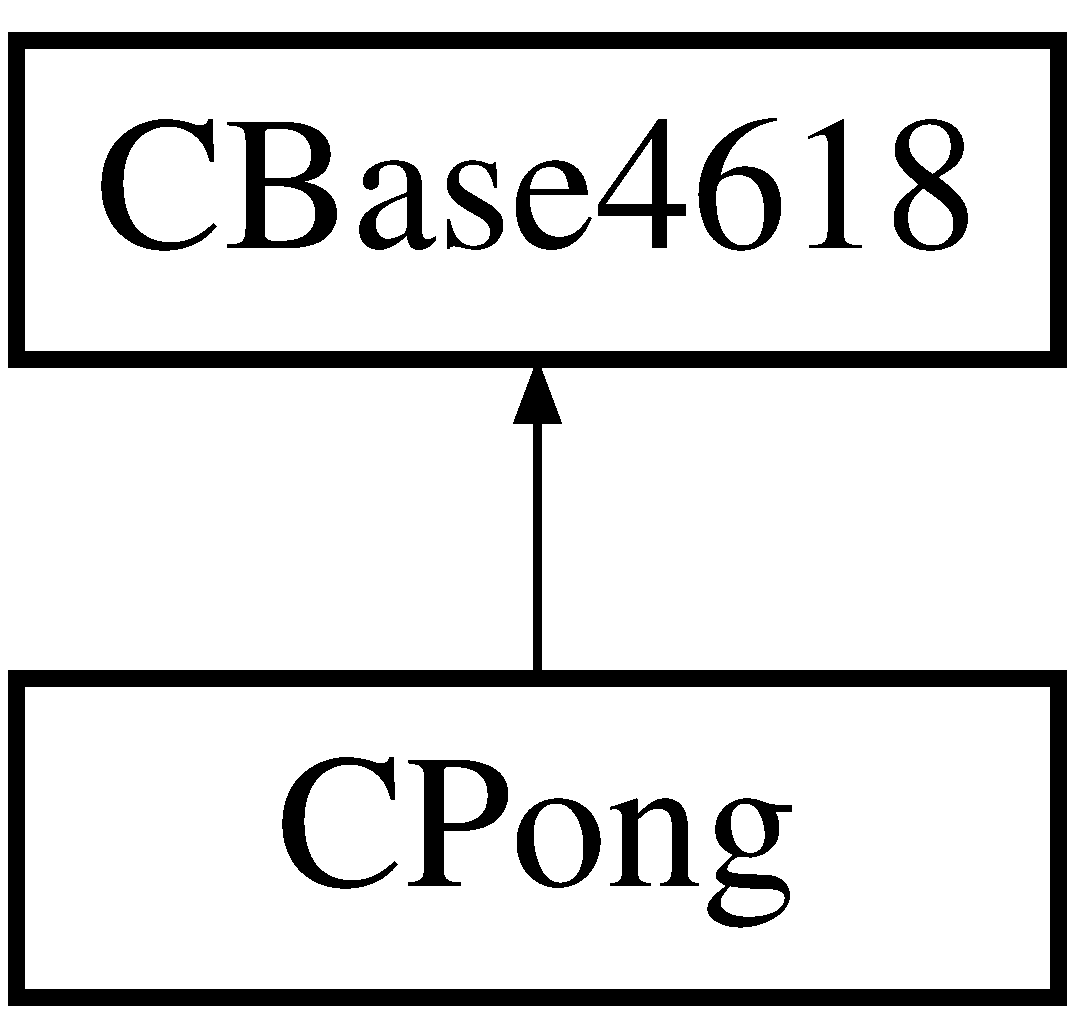
\includegraphics[height=2.000000cm]{class_c_pong}
\end{center}
\end{figure}
\subsection*{Public Member Functions}
\begin{DoxyCompactItemize}
\item 
void \hyperlink{class_c_pong_a819c9942552ff12a11be284a89e3ab12}{update} () override
\begin{DoxyCompactList}\small\item\em G\+E\+TS J\+O\+Y\+S\+T\+I\+CK I\+N\+P\+UT. \end{DoxyCompactList}\item 
void \hyperlink{class_c_pong_af43dbb61f1f1addd6920b01aeca3fa63}{draw} () override
\begin{DoxyCompactList}\small\item\em renders all the graphics on the screen. \end{DoxyCompactList}\item 
void \hyperlink{class_c_pong_a0fa724d6d3dc8e65decb1276a4a1c38a}{reset} ()
\begin{DoxyCompactList}\small\item\em resets the position velocity to default. \end{DoxyCompactList}\end{DoxyCompactItemize}
\subsection*{Public Attributes}
\begin{DoxyCompactItemize}
\item 
\hypertarget{class_c_pong_a1dae5c9ec589eb86e275a0470095f530}{}\label{class_c_pong_a1dae5c9ec589eb86e275a0470095f530} 
int \hyperlink{class_c_pong_a1dae5c9ec589eb86e275a0470095f530}{y\+\_\+pos}
\begin{DoxyCompactList}\small\item\em Y value Jo\+Y\+S\+T\+I\+CK. \end{DoxyCompactList}\item 
\hypertarget{class_c_pong_a3aa66544f80bed43ebffeb3c2711521e}{}\label{class_c_pong_a3aa66544f80bed43ebffeb3c2711521e} 
const int \hyperlink{class_c_pong_a3aa66544f80bed43ebffeb3c2711521e}{frame\+Delay} = 1000 / 26
\begin{DoxyCompactList}\small\item\em 33ms delay \end{DoxyCompactList}\item 
\hypertarget{class_c_pong_a460ef9c18d512e61e8b277aaf9c2db12}{}\label{class_c_pong_a460ef9c18d512e61e8b277aaf9c2db12} 
uint32\+\_\+t \hyperlink{class_c_pong_a460ef9c18d512e61e8b277aaf9c2db12}{frame\+Start}
\begin{DoxyCompactList}\small\item\em start time. \end{DoxyCompactList}\item 
\hypertarget{class_c_pong_a1432a4e6bcd2cfc7eb567e9c5dc2f136}{}\label{class_c_pong_a1432a4e6bcd2cfc7eb567e9c5dc2f136} 
double \hyperlink{class_c_pong_a1432a4e6bcd2cfc7eb567e9c5dc2f136}{last}
\begin{DoxyCompactList}\small\item\em previous time \end{DoxyCompactList}\item 
\hypertarget{class_c_pong_aa9bb35ee26e1722e574f8629d381445b}{}\label{class_c_pong_aa9bb35ee26e1722e574f8629d381445b} 
int \hyperlink{class_c_pong_aa9bb35ee26e1722e574f8629d381445b}{score}
\begin{DoxyCompactList}\small\item\em score of player \end{DoxyCompactList}\item 
\hypertarget{class_c_pong_a2da2c577ed7dd0ecea96221c3dd4e5a4}{}\label{class_c_pong_a2da2c577ed7dd0ecea96221c3dd4e5a4} 
int \hyperlink{class_c_pong_a2da2c577ed7dd0ecea96221c3dd4e5a4}{press}
\begin{DoxyCompactList}\small\item\em button output value \end{DoxyCompactList}\end{DoxyCompactItemize}


\subsection{Detailed Description}
C++ object used to create a Pong;. 

This class drwas and updates the paddles on the screen Y axis input comes from the joystck.

\begin{DoxyAuthor}{Author}
Balkaran Sidhu 
\end{DoxyAuthor}


\subsection{Member Function Documentation}
\hypertarget{class_c_pong_af43dbb61f1f1addd6920b01aeca3fa63}{}\label{class_c_pong_af43dbb61f1f1addd6920b01aeca3fa63} 
\index{C\+Pong@{C\+Pong}!draw@{draw}}
\index{draw@{draw}!C\+Pong@{C\+Pong}}
\subsubsection{\texorpdfstring{draw()}{draw()}}
{\footnotesize\ttfamily void C\+Pong\+::draw (\begin{DoxyParamCaption}{ }\end{DoxyParamCaption})\hspace{0.3cm}{\ttfamily [override]}, {\ttfamily [virtual]}}



renders all the graphics on the screen. 


\begin{DoxyParams}{Parameters}
{\em N\+O\+N\+E.} & \\
\hline
\end{DoxyParams}
\begin{DoxyReturn}{Returns}
nothing to return 
\end{DoxyReturn}


Reimplemented from \hyperlink{class_c_base4618_a853327d563d064bb31db241861c4d291}{C\+Base4618}.

\hypertarget{class_c_pong_a0fa724d6d3dc8e65decb1276a4a1c38a}{}\label{class_c_pong_a0fa724d6d3dc8e65decb1276a4a1c38a} 
\index{C\+Pong@{C\+Pong}!reset@{reset}}
\index{reset@{reset}!C\+Pong@{C\+Pong}}
\subsubsection{\texorpdfstring{reset()}{reset()}}
{\footnotesize\ttfamily void C\+Pong\+::reset (\begin{DoxyParamCaption}{ }\end{DoxyParamCaption})}



resets the position velocity to default. 


\begin{DoxyParams}{Parameters}
{\em N\+O\+NE} & \\
\hline
\end{DoxyParams}
\begin{DoxyReturn}{Returns}
nothing to return 
\end{DoxyReturn}
\hypertarget{class_c_pong_a819c9942552ff12a11be284a89e3ab12}{}\label{class_c_pong_a819c9942552ff12a11be284a89e3ab12} 
\index{C\+Pong@{C\+Pong}!update@{update}}
\index{update@{update}!C\+Pong@{C\+Pong}}
\subsubsection{\texorpdfstring{update()}{update()}}
{\footnotesize\ttfamily void C\+Pong\+::update (\begin{DoxyParamCaption}{ }\end{DoxyParamCaption})\hspace{0.3cm}{\ttfamily [override]}, {\ttfamily [virtual]}}



G\+E\+TS J\+O\+Y\+S\+T\+I\+CK I\+N\+P\+UT. 


\begin{DoxyParams}{Parameters}
{\em N\+O\+N\+E.} & \\
\hline
\end{DoxyParams}
\begin{DoxyReturn}{Returns}
nothing to return 
\end{DoxyReturn}


Reimplemented from \hyperlink{class_c_base4618_ae1ac81eaa56ded6600262c361f723cb8}{C\+Base4618}.



The documentation for this class was generated from the following files\+:\begin{DoxyCompactItemize}
\item 
C\+Pong.\+h\item 
C\+Pong.\+cpp\end{DoxyCompactItemize}

\hypertarget{class_serial}{}\section{Serial Class Reference}
\label{class_serial}\index{Serial@{Serial}}
\subsection*{Public Member Functions}
\begin{DoxyCompactItemize}
\item 
\hypertarget{class_serial_a599d3e220888815b8da436ea45a5c655}{}\label{class_serial_a599d3e220888815b8da436ea45a5c655} 
bool {\bfseries open} (std\+::string comm\+Port\+Name, int bit\+Rate=115200)
\item 
int \hyperlink{class_serial_aae3d630a4fd81c8b148cb4eebdb91392}{write} (const char $\ast$buffer, int buff\+Len)
\item 
int \hyperlink{class_serial_a8266889eb5bfa7ef8b53595c5482133d}{read} (char $\ast$buffer, int buff\+Len)
\item 
\hypertarget{class_serial_a63b7abf172cad25bfc998b3b1f98310f}{}\label{class_serial_a63b7abf172cad25bfc998b3b1f98310f} 
void {\bfseries flush} ()
\end{DoxyCompactItemize}


\subsection{Member Function Documentation}
\hypertarget{class_serial_a8266889eb5bfa7ef8b53595c5482133d}{}\label{class_serial_a8266889eb5bfa7ef8b53595c5482133d} 
\index{Serial@{Serial}!read@{read}}
\index{read@{read}!Serial@{Serial}}
\subsubsection{\texorpdfstring{read()}{read()}}
{\footnotesize\ttfamily int Serial\+::read (\begin{DoxyParamCaption}\item[{char $\ast$}]{buffer,  }\item[{int}]{buff\+Len }\end{DoxyParamCaption})}

Reads a string of bytes from the serial port.


\begin{DoxyParams}{Parameters}
{\em buffer} & pointer to the buffer to be written to \\
\hline
{\em buff\+Len} & the size of the buffer\\
\hline
\end{DoxyParams}
\begin{DoxyReturn}{Returns}
int the number of bytes read 
\end{DoxyReturn}
\hypertarget{class_serial_aae3d630a4fd81c8b148cb4eebdb91392}{}\label{class_serial_aae3d630a4fd81c8b148cb4eebdb91392} 
\index{Serial@{Serial}!write@{write}}
\index{write@{write}!Serial@{Serial}}
\subsubsection{\texorpdfstring{write()}{write()}}
{\footnotesize\ttfamily int Serial\+::write (\begin{DoxyParamCaption}\item[{const char $\ast$}]{buffer,  }\item[{int}]{buff\+Len }\end{DoxyParamCaption})}

Writes a string of bytes to the serial port.


\begin{DoxyParams}{Parameters}
{\em buffer} & pointer to the buffer containing the bytes \\
\hline
{\em buff\+Len} & the number of bytes in the buffer\\
\hline
\end{DoxyParams}
\begin{DoxyReturn}{Returns}
int the number of bytes written 
\end{DoxyReturn}


The documentation for this class was generated from the following files\+:\begin{DoxyCompactItemize}
\item 
Serial.\+h\item 
Serial.\+cpp\end{DoxyCompactItemize}

\hypertarget{class_server}{}\section{Server Class Reference}
\label{class_server}\index{Server@{Server}}
\subsection*{Public Member Functions}
\begin{DoxyCompactItemize}
\item 
\hypertarget{class_server_a7ebba75484fe844bb3e2920205455a74}{}\label{class_server_a7ebba75484fe844bb3e2920205455a74} 
void {\bfseries start} (int port)
\item 
\hypertarget{class_server_ad49615121ae4496bb6f8248530937101}{}\label{class_server_ad49615121ae4496bb6f8248530937101} 
void {\bfseries set\+\_\+txim} (cv\+::\+Mat \&im)
\item 
\hypertarget{class_server_ad01a77ea78115b7e6fc0603e0f239963}{}\label{class_server_ad01a77ea78115b7e6fc0603e0f239963} 
void {\bfseries get\+\_\+cmd} (std\+::vector$<$ std\+::string $>$ \&cmds)
\end{DoxyCompactItemize}


The documentation for this class was generated from the following files\+:\begin{DoxyCompactItemize}
\item 
server.\+h\item 
server.\+cpp\end{DoxyCompactItemize}

%--- End generated contents ---

% Index
\backmatter
\newpage
\phantomsection
\clearemptydoublepage
\addcontentsline{toc}{chapter}{Index}
\printindex

\end{document}
